%%%%%%%%%%%%%%%%%%%%%%%%%%%%%%%%%%%%%%%%%
% Jacobs Landscape Poster
% LaTeX Template
% Version 1.0 (29/03/13)
%
% Created by:
% Computational Physics and Biophysics Group, Jacobs University
% https://teamwork.jacobs-university.de:8443/confluence/display/CoPandBiG/LaTeX+Poster
% 
% Further modified by:
% Nathaniel Johnston (nathaniel@njohnston.ca)
%
% This template has been downloaded from:
% http://www.LaTeXTemplates.com
%
% License:
% CC BY-NC-SA 3.0 (http://creativecommons.org/licenses/by-nc-sa/3.0/)
%
%%%%%%%%%%%%%%%%%%%%%%%%%%%%%%%%%%%%%%%%%

%----------------------------------------------------------------------------------------
% PACKAGES AND OTHER DOCUMENT CONFIGURATIONS
%----------------------------------------------------------------------------------------
  \documentclass[final]{beamer}

  \usepackage[scale=1.2]{beamerposter} % Use the beamerposter package for laying out the poster
  \usepackage{mathtools,amsmath}


  \usetheme{confposter} % Use the confposter theme supplied with this template
  \setbeamercolor{block example title}{fg=white,bg=calblue}
  \setbeamercolor{block title}{fg=calblue,bg=white} % Colors of the block titles
  \setbeamercolor{block body}{fg=black,bg=white} % Colors of the body of blocks
  \setbeamercolor{block alerted title}{fg=white,bg=calblue!70} % Colors of the highlighted block titles
  \setbeamercolor{block alerted body}{fg=black,bg=calblue!10} % Colors of the body of highlighted blocks
  \setbeamertemplate{itemize item}[triangle]
  \setbeamertemplate{caption}[numbered]
  % Many more colors are available for use in beamerthemeconfposter.sty

  %-----------------------------------------------------------
  % Define the column widths and overall poster size
  % To set effective sepwid, onecolwid and twocolwid values, first choose how many columns you want and how much separation you want between columns
  % In this template, the separation width chosen is 0.024 of the paper width and a 4-column layout
  % onecolwid should therefore be (1-(# of columns+1)*sepwid)/# of columns e.g. (1-(4+1)*0.024)/4 = 0.22
  % Set twocolwid to be (2*onecolwid)+sepwid = 0.464
  % Set threecolwid to be (3*onecolwid)+2*sepwid = 0.708

  \newlength{\sepwid}
  \newlength{\onecolwid}
  \newlength{\twocolwid}
  \newlength{\threecolwid}
  \setlength{\paperwidth}{48in} % A0 width: 46.8in
  \setlength{\paperheight}{36in} % A0 height: 33.1in
  \setlength{\sepwid}{0.024\paperwidth} % Separation width (white space) between columns
  \setlength{\onecolwid}{0.22\paperwidth} % Width of one column
  \setlength{\twocolwid}{0.464\paperwidth} % Width of two columns
  \setlength{\threecolwid}{0.708\paperwidth} % Width of three columns
  \setlength{\topmargin}{-0.5in} % Reduce the top margin size
  %-----------------------------------------------------------

  \usepackage{graphicx}  % Required for including images
  \usepackage{booktabs} % Top and bottom rules for tables
  % \usepackage{apacite}
  \usepackage{wrapfig}
  \usepackage{amssymb,amsmath,amsthm,amsfonts}
  \usepackage{tikz}
  \usepackage{caption}
  \usepackage{listings}
  \usepackage{fancyvrb}
  \usepackage{subcaption}
  \usepackage{natbib}
  \usepackage{minted}
  \captionsetup{font=normalsize, labelfont=normalsize}

  % \setlength{\parskip}{10cm}

\newcommand{\first}{\textsuperscript{1}}
\title{Mouselab-MDP: A new paradigm for tracing how people plan}

% \author{Frederick Callaway, Falk Lieder, Paul M. Krueger, and Thomas L. Griffiths}

\author{Frederick Callaway\first^*, Falk Lieder\first, Paul M. Krueger\first, and Thomas L. Griffiths}
\institute{University of California, Berkeley \\ {\bf \first} {\small These authors contributed equally.\quad \textsuperscript{*} Correspondance: fredcallaway@berkeley.edu}}

\begin{document}

% Logos
\addtobeamertemplate{headline}{}
{\begin{tikzpicture}[remember picture, overlay]
  \node [anchor=north east, inner sep=2cm]  at (current page.north east)
  {
\includegraphics[height=8cm]{berkeley.png}};
  \node [anchor=north west, inner sep=2cm]  at (current page.north west)
  {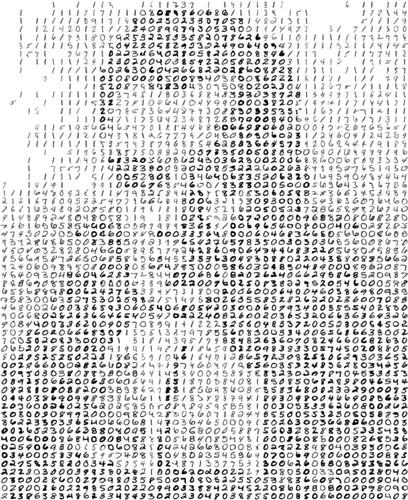
\includegraphics[height=8cm]{cocosci.jpg}};
\end{tikzpicture}}

\addtobeamertemplate{block end}{}{\vspace*{2ex}} % White space under blocks
\addtobeamertemplate{block alerted end}{}{\vspace*{2ex}} % White space under highlighted (alert) blocks
\setlength{\belowcaptionskip}{2ex} % White space under figures
\setlength\belowdisplayshortskip{2ex} % White space under equations

\begin{frame}[t, fragile] % The whole poster is enclosed in one beamer frame
\begin{columns}[t] % The whole poster consists of three major columns, the second of which is split into two columns twice
\begin{column}{\sepwid}\end{column} % Empty spacer column

%----------------------------------------------------------------------------------------
% CONTENT
%----------------------------------------------------------------------------------------

\begin{column}{\onecolwid} % Begin column 1
  \begin{block}{Key points}\label{contribution}
    \begin{itemize}
      \item Planning is an unobservable cognitive process.
      %\item Studying unobservable things is hard.
      \item We introduce a novel paradigm that makes planning visible by tracking which states and transitions people inspect and in which order.
      \item This data sheds new light on pruning.
      \item We release the paradigm open-source as a jsPsych plugin \cite{DeLeeuw2015}: \texttt{https://github.com/fredcallaway/Mouselab-MDP}
    \end{itemize}
    % The flexible configuration allows researchers to create a wide variety of experiments with minimal programming effort.
  \end{block}

  % \begin{alertblock}{Key findings}\label{key-findings}
  %   \textbf{Sparse pseudo-rewards} can
  %   \begin{itemize}
  %     \item lead to \textbf{optimal behavior} in a \textbf{limited-depth planner}.
  %     \item induce \textbf{goal directed planning} in humans.
  %     \item \textbf{improve human decision making}.
  %   \end{itemize}
  % \end{alertblock}

  \begin{block}{Background}\label{Background}
    \begin{itemize}
      \item Many problems require planning into the distant future.
            %Brute force search is intractable, thus people must rely on \textbf{approximate planning strategies}.
            Previous work has identified %abstract
            \textbf{approximate planning strategies} based on patterns of human errors \cite{Huys2015}.
      \item \textbf{Process-tracing paradigms} externalize cognitive processes.
            To trace decision strategies, the ``Mouselab'' paradigm \cite{Payne1988} requires people to click on cells of a payoff matrix to reveal the outcomes. We apply this idea to MDPs.
    \end{itemize}

    

  \end{block}

  \begin{block}{Example code}\label{usage}
    This CofeeScript code generates Fig.~\ref{fig:simple}.
    % \begin{Verbatim}[fontsize=\small]
    \begin{minted}[fontsize=\small]{coffee}
trial =  # a trial is defined by a JS object
  type: 'mouselab-mdp'  # use the jsPsych plugin
  graph:  # defines transition and reward functions
    B:
      up: [5, 'A']  # action: [reward, next_state]
      down: [-5, 'C']
    A: {}  # terminal states have no actions
    C: {}
  layout:  # defines position of states
    A: [1, 1]
    B: [1, 2]
    C: [1, 3]
  initial: 'B'  # initial state of player
  stateLabels: {A: 'A', B: 'B', C: 'C'}
  stateDisplay: 'always'  # never, hover, click, always
  edgeLabels: 'reward'  # can be an arbitrary mapping
  edgeDisplay: 'click'  # never, hover, click, always
  edgeClickCost: 1  # subtracted from score whenever
                    # an edge is clicked
    \end{minted}{coffee}
    % \end{Verbatim}
  \end{block}

\end{column} % End column 1
%------------------------------------------------------------------------------

\begin{column}{\sepwid}\end{column} % Empty spacer column
\begin{column}{\twocolwid} % Begin column 2
  \vspace{-1cm}
  \begin{figure}
    \label{fig:main}
    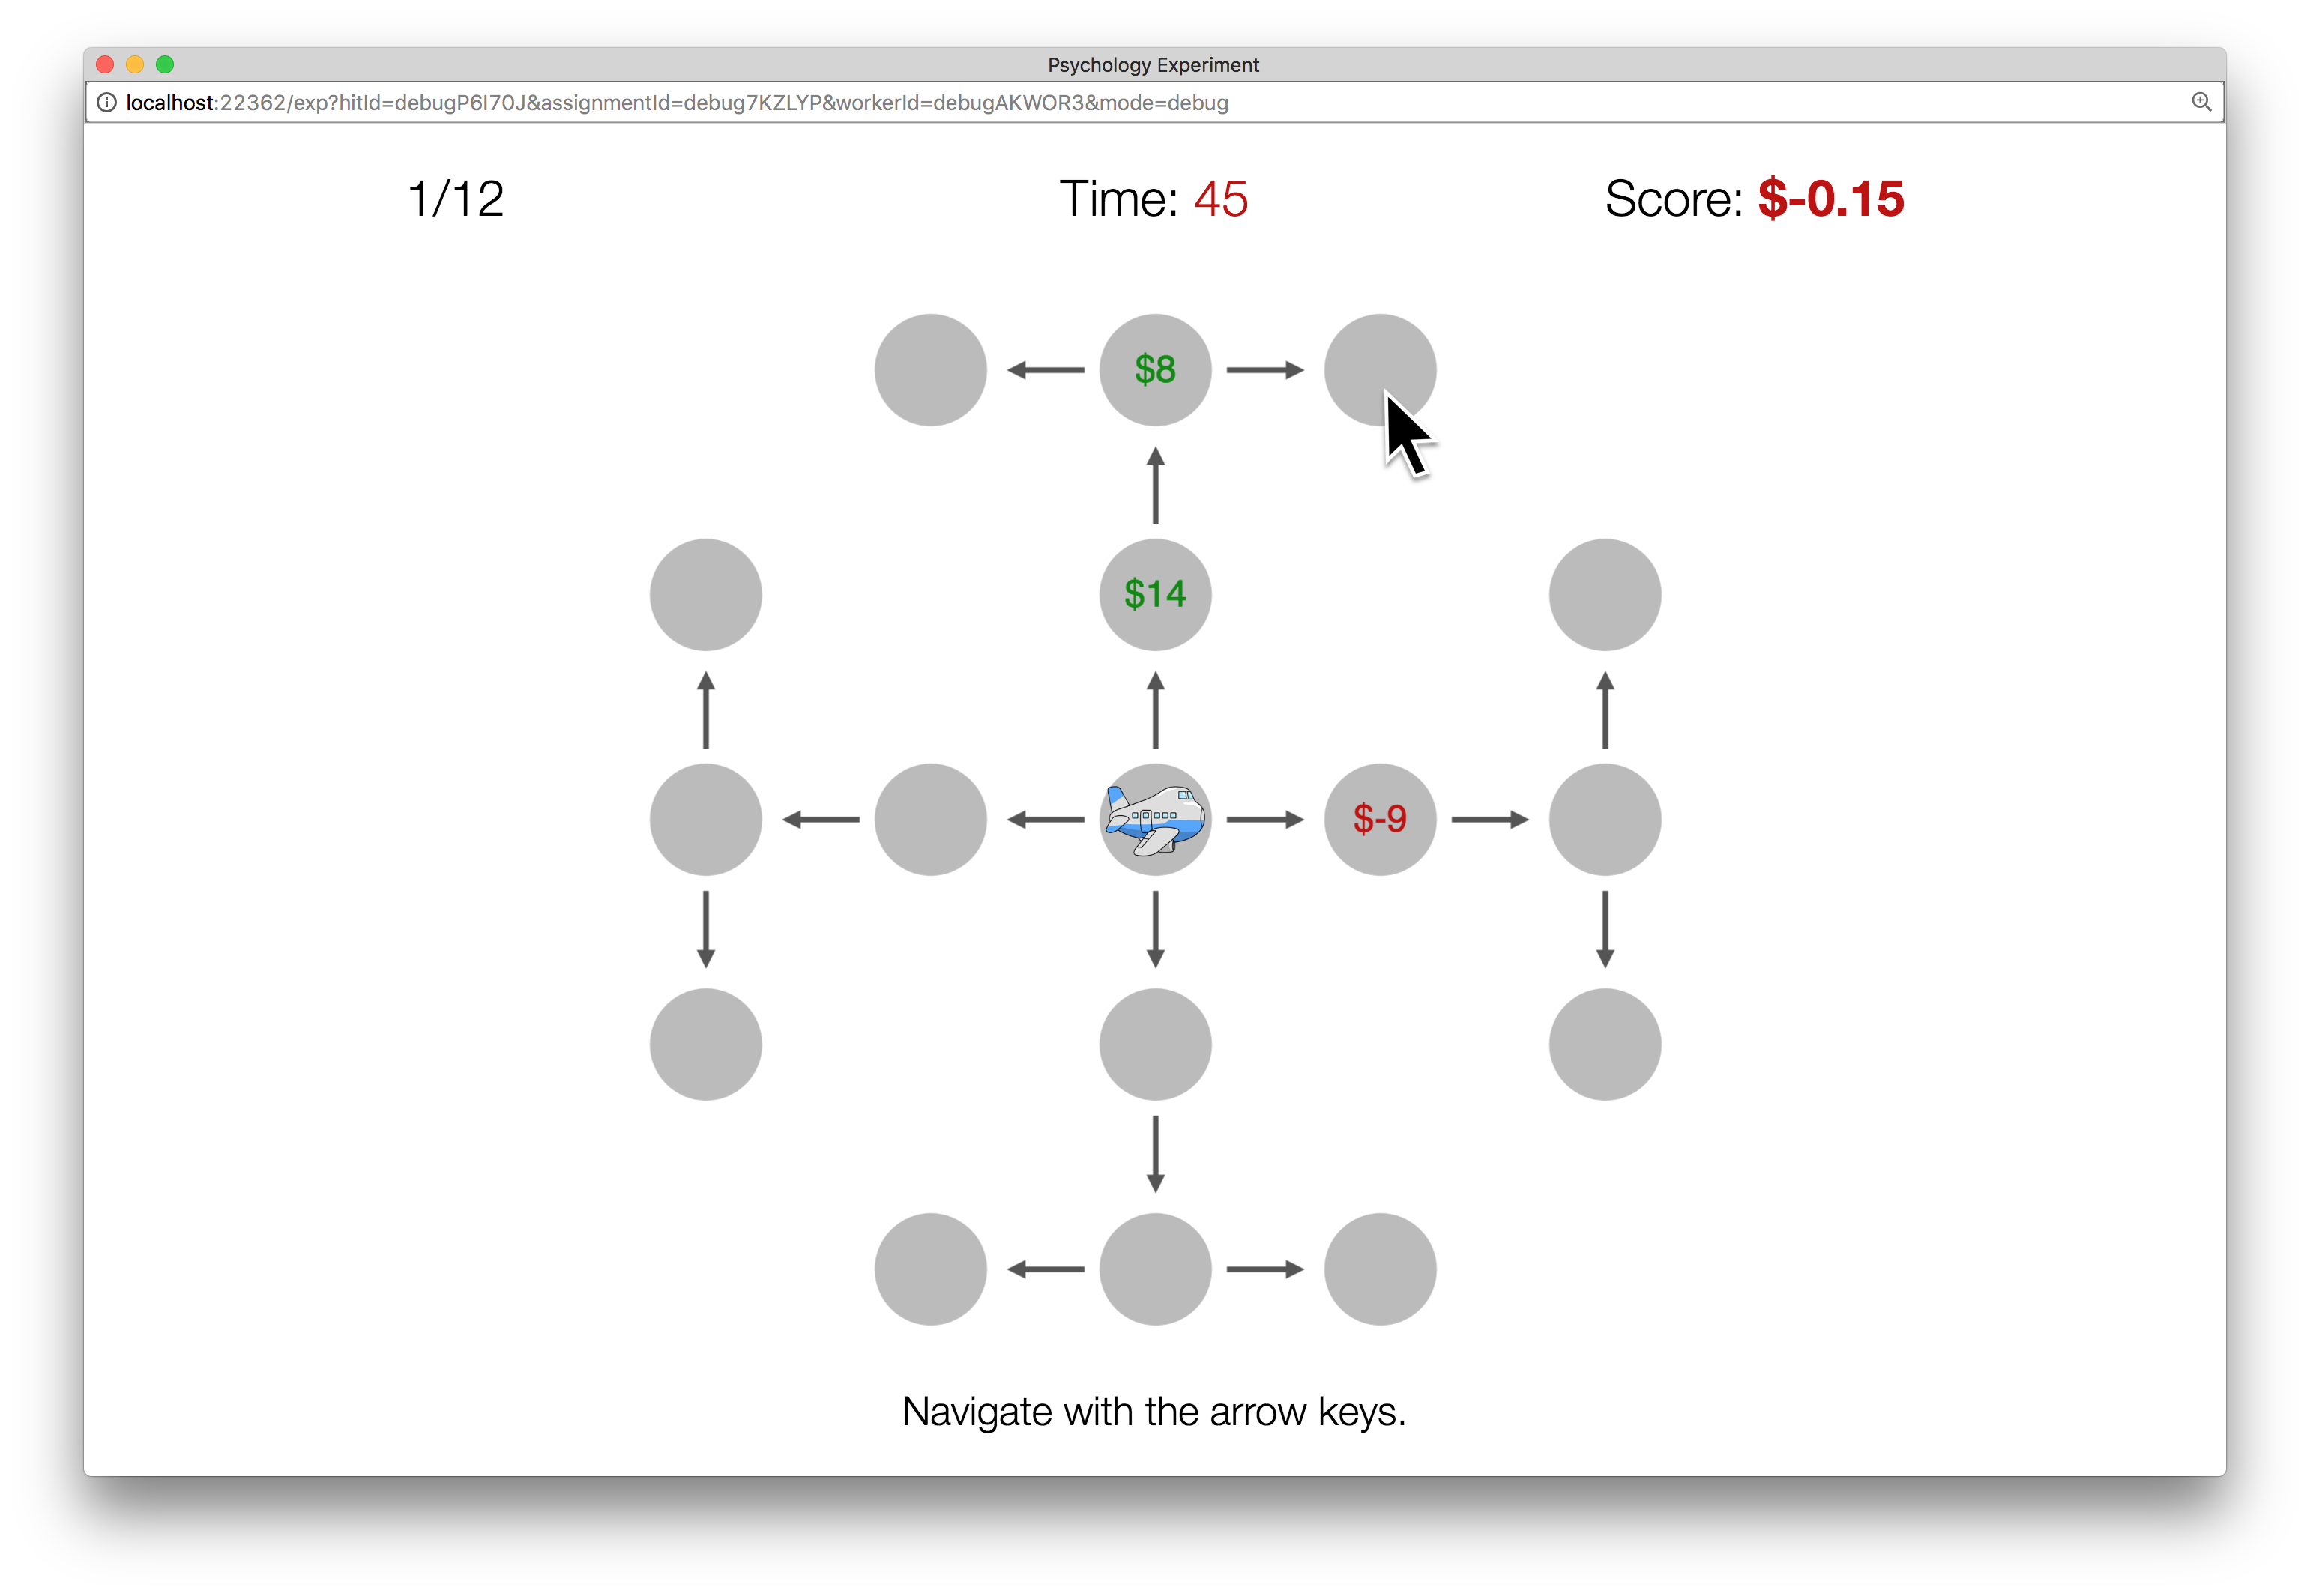
\includegraphics[width=0.85\linewidth]{figs/example1.png}
    % \captionsetup{width=0.9\linewidth}
    % \caption[first]{Web of Cash experimental interface.}
  \end{figure}

  \vspace{-1cm}

  \begin{figure}
    \centering
    \begin{subfigure}{.28\textwidth}
      \centering
      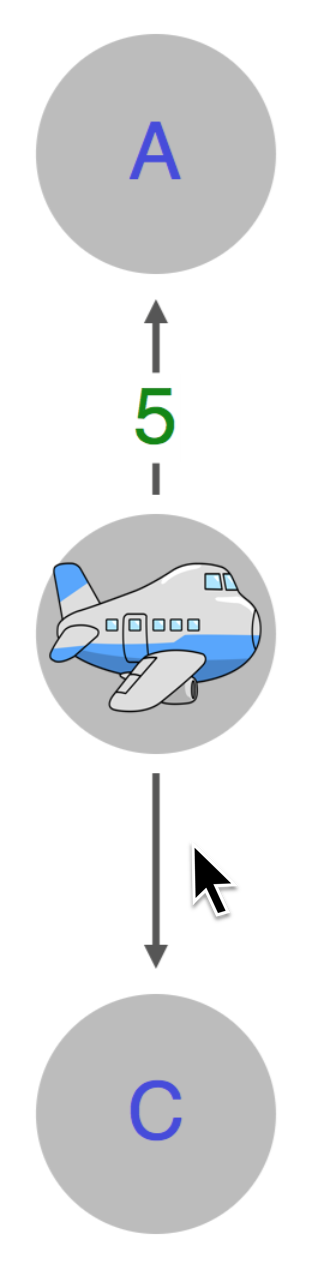
\includegraphics[height=10cm]{figs/simple.png}
      \caption{}
      \label{fig:simple}
    \end{subfigure}
    \begin{subfigure}{.38\textwidth}
      \centering
      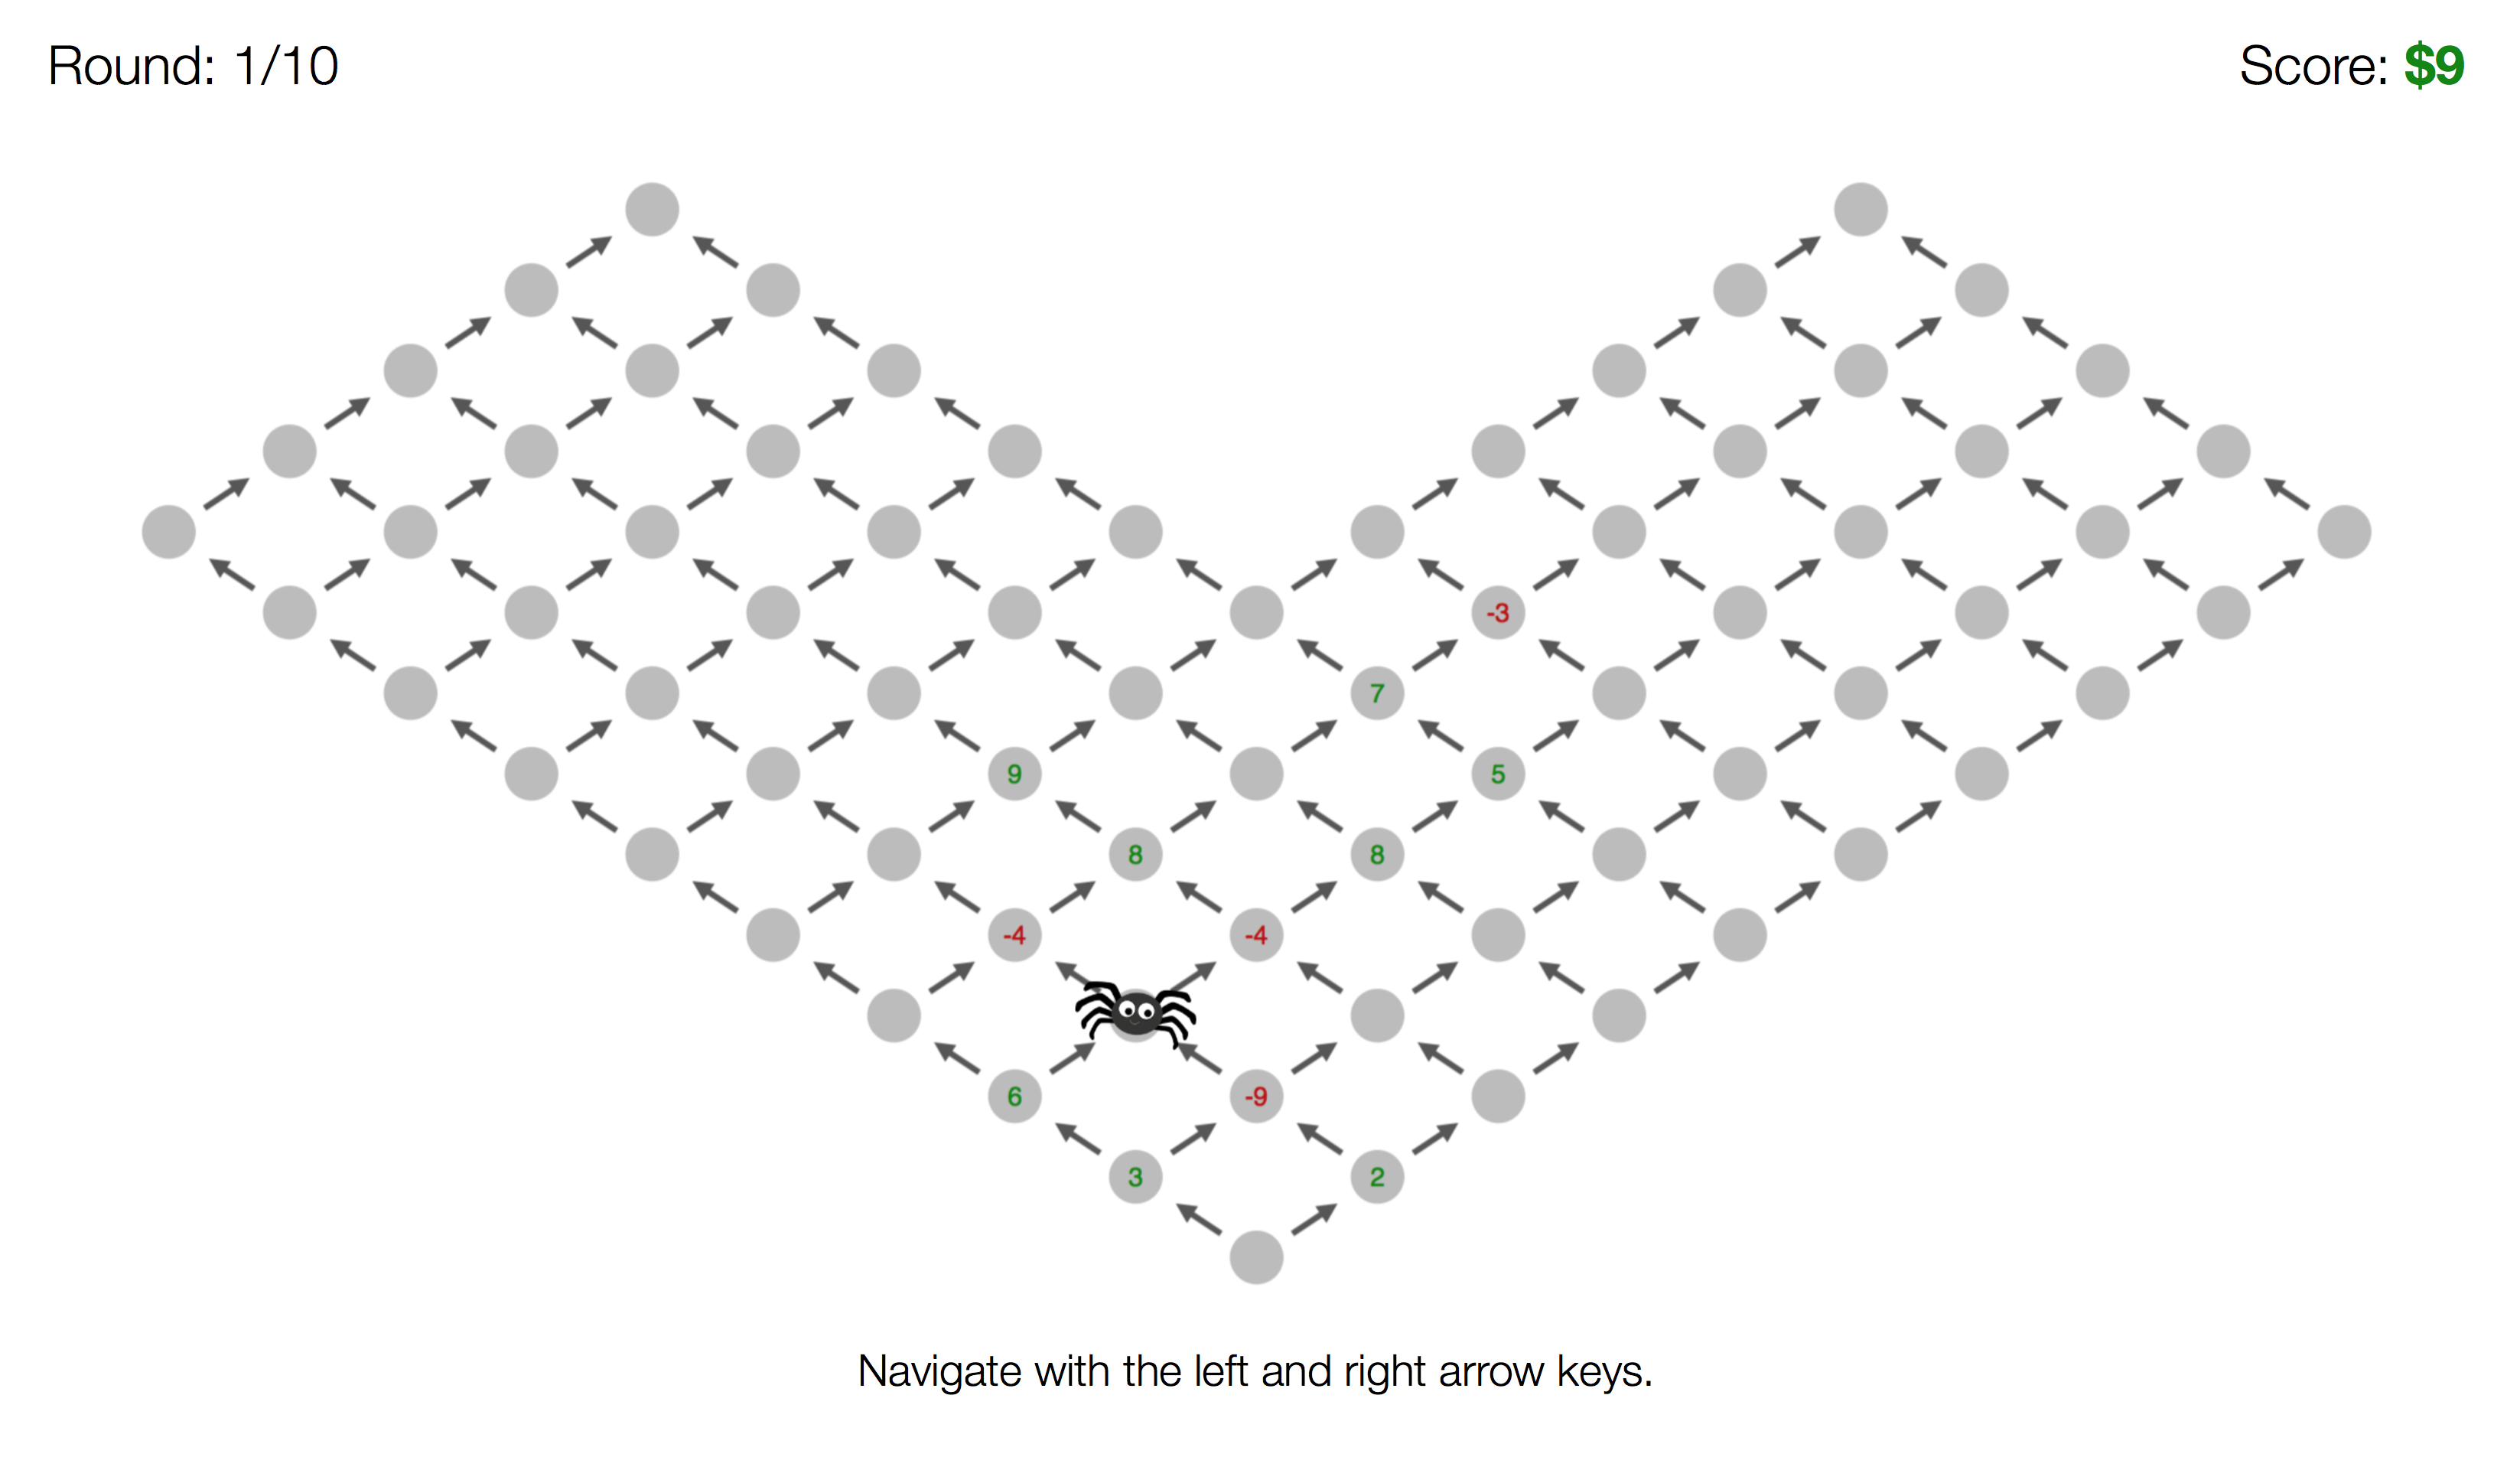
\includegraphics[height=10cm]{figs/heart.png}
      \caption{}
      \label{fig:heart}
    \end{subfigure}
    \begin{subfigure}{.28\textwidth}
      \centering
      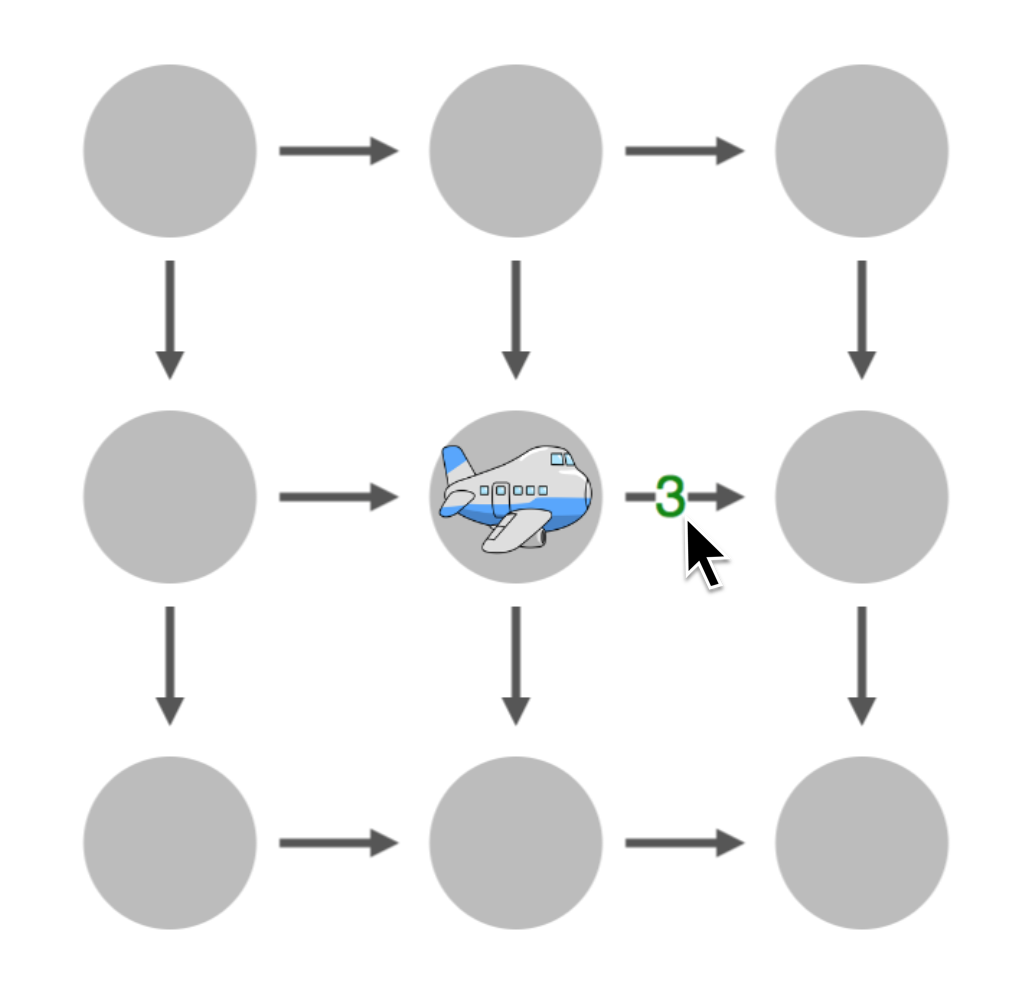
\includegraphics[height=10cm]{figs/grid2.png}
      \caption{}
      \label{fig:hover}
    \end{subfigure}
    \caption{(a) See \textbf{Example code}; (b) a programatically generated layout; (c) rewards displayed on hover.}
    \label{fig:test}
  \end{figure}


  \begin{figure}
    \centering
    \begin{subfigure}{0.48\textwidth}
      \centering
      \label{fig:click_heat}
      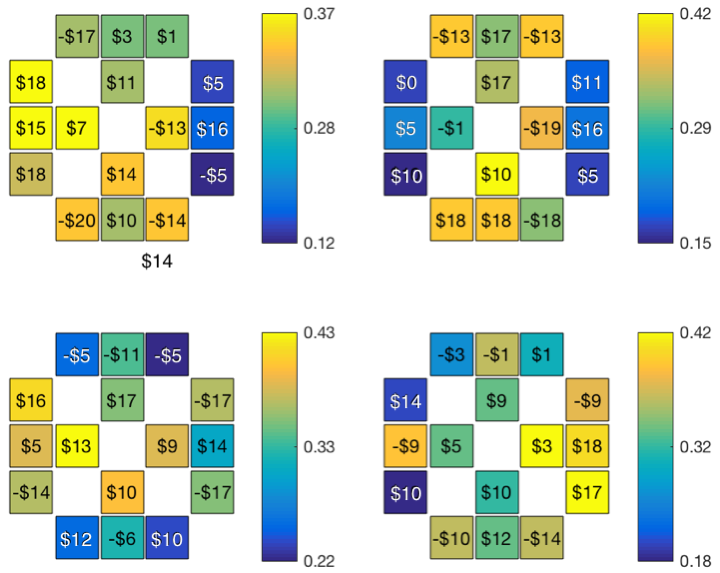
\includegraphics[width=0.9\linewidth]{figs/click_locations_noFB_before1stFlight_small.png}
      \caption{}
    \end{subfigure}
    \begin{subfigure}{0.48\textwidth}
      \centering
      \label{fig:click_sets}
      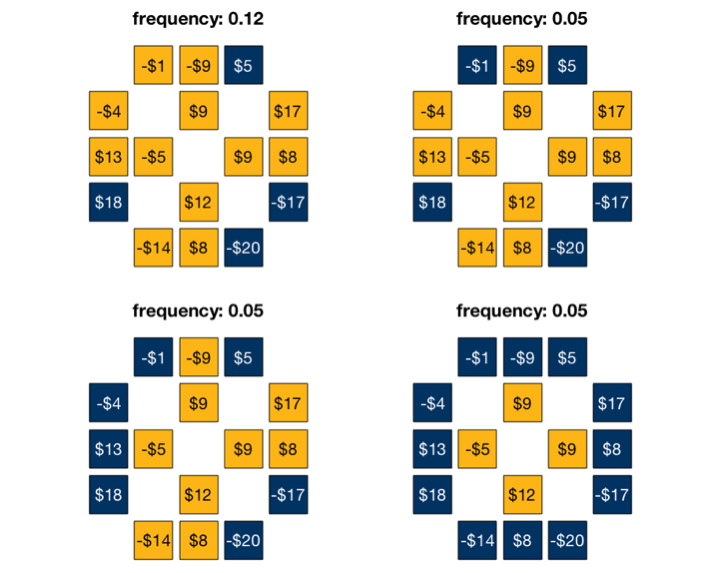
\includegraphics[width=0.9\linewidth]{figs/click_sets_trial4_noFB_small.png}
      \caption{}
    \end{subfigure}
    % \captionsetup{width=0.9\linewidth}
    \caption[first]{Human clicking patterns reveal pruning strategies. Each subplot shows the location and monetary value of each state. (a) Colors indicate how often each state was inspected before the first move, for four MDPs. (b) The four most common click sets for one MDP. Inspected states are gold.}
  \end{figure}


  % \begin{figure}
  %   \centering
  %   \begin{minipage}{.3\textwidth}
  %     \centering
  %     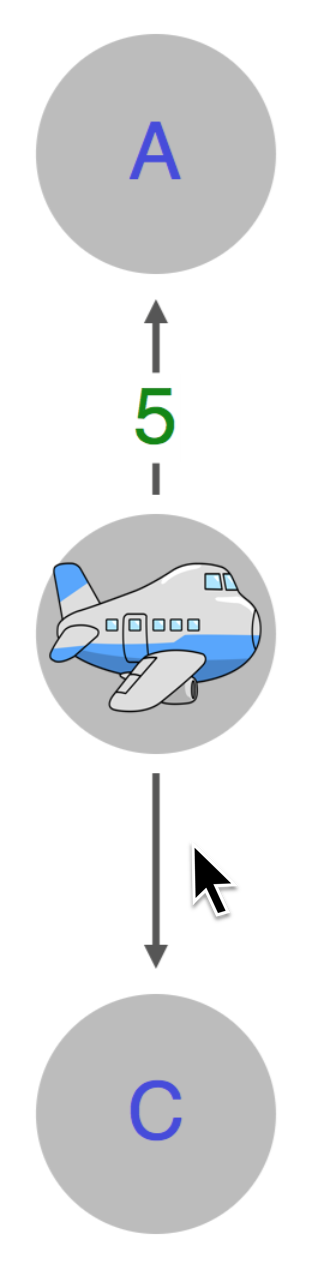
\includegraphics[height=10cm]{figs/simple.png}
  %     \captionof{figure}{Example from \textbf{Usage}}
  %     \label{fig:simple}
  %   \end{minipage}%
  %   \begin{minipage}{.4\textwidth}
  %     \centering
  %     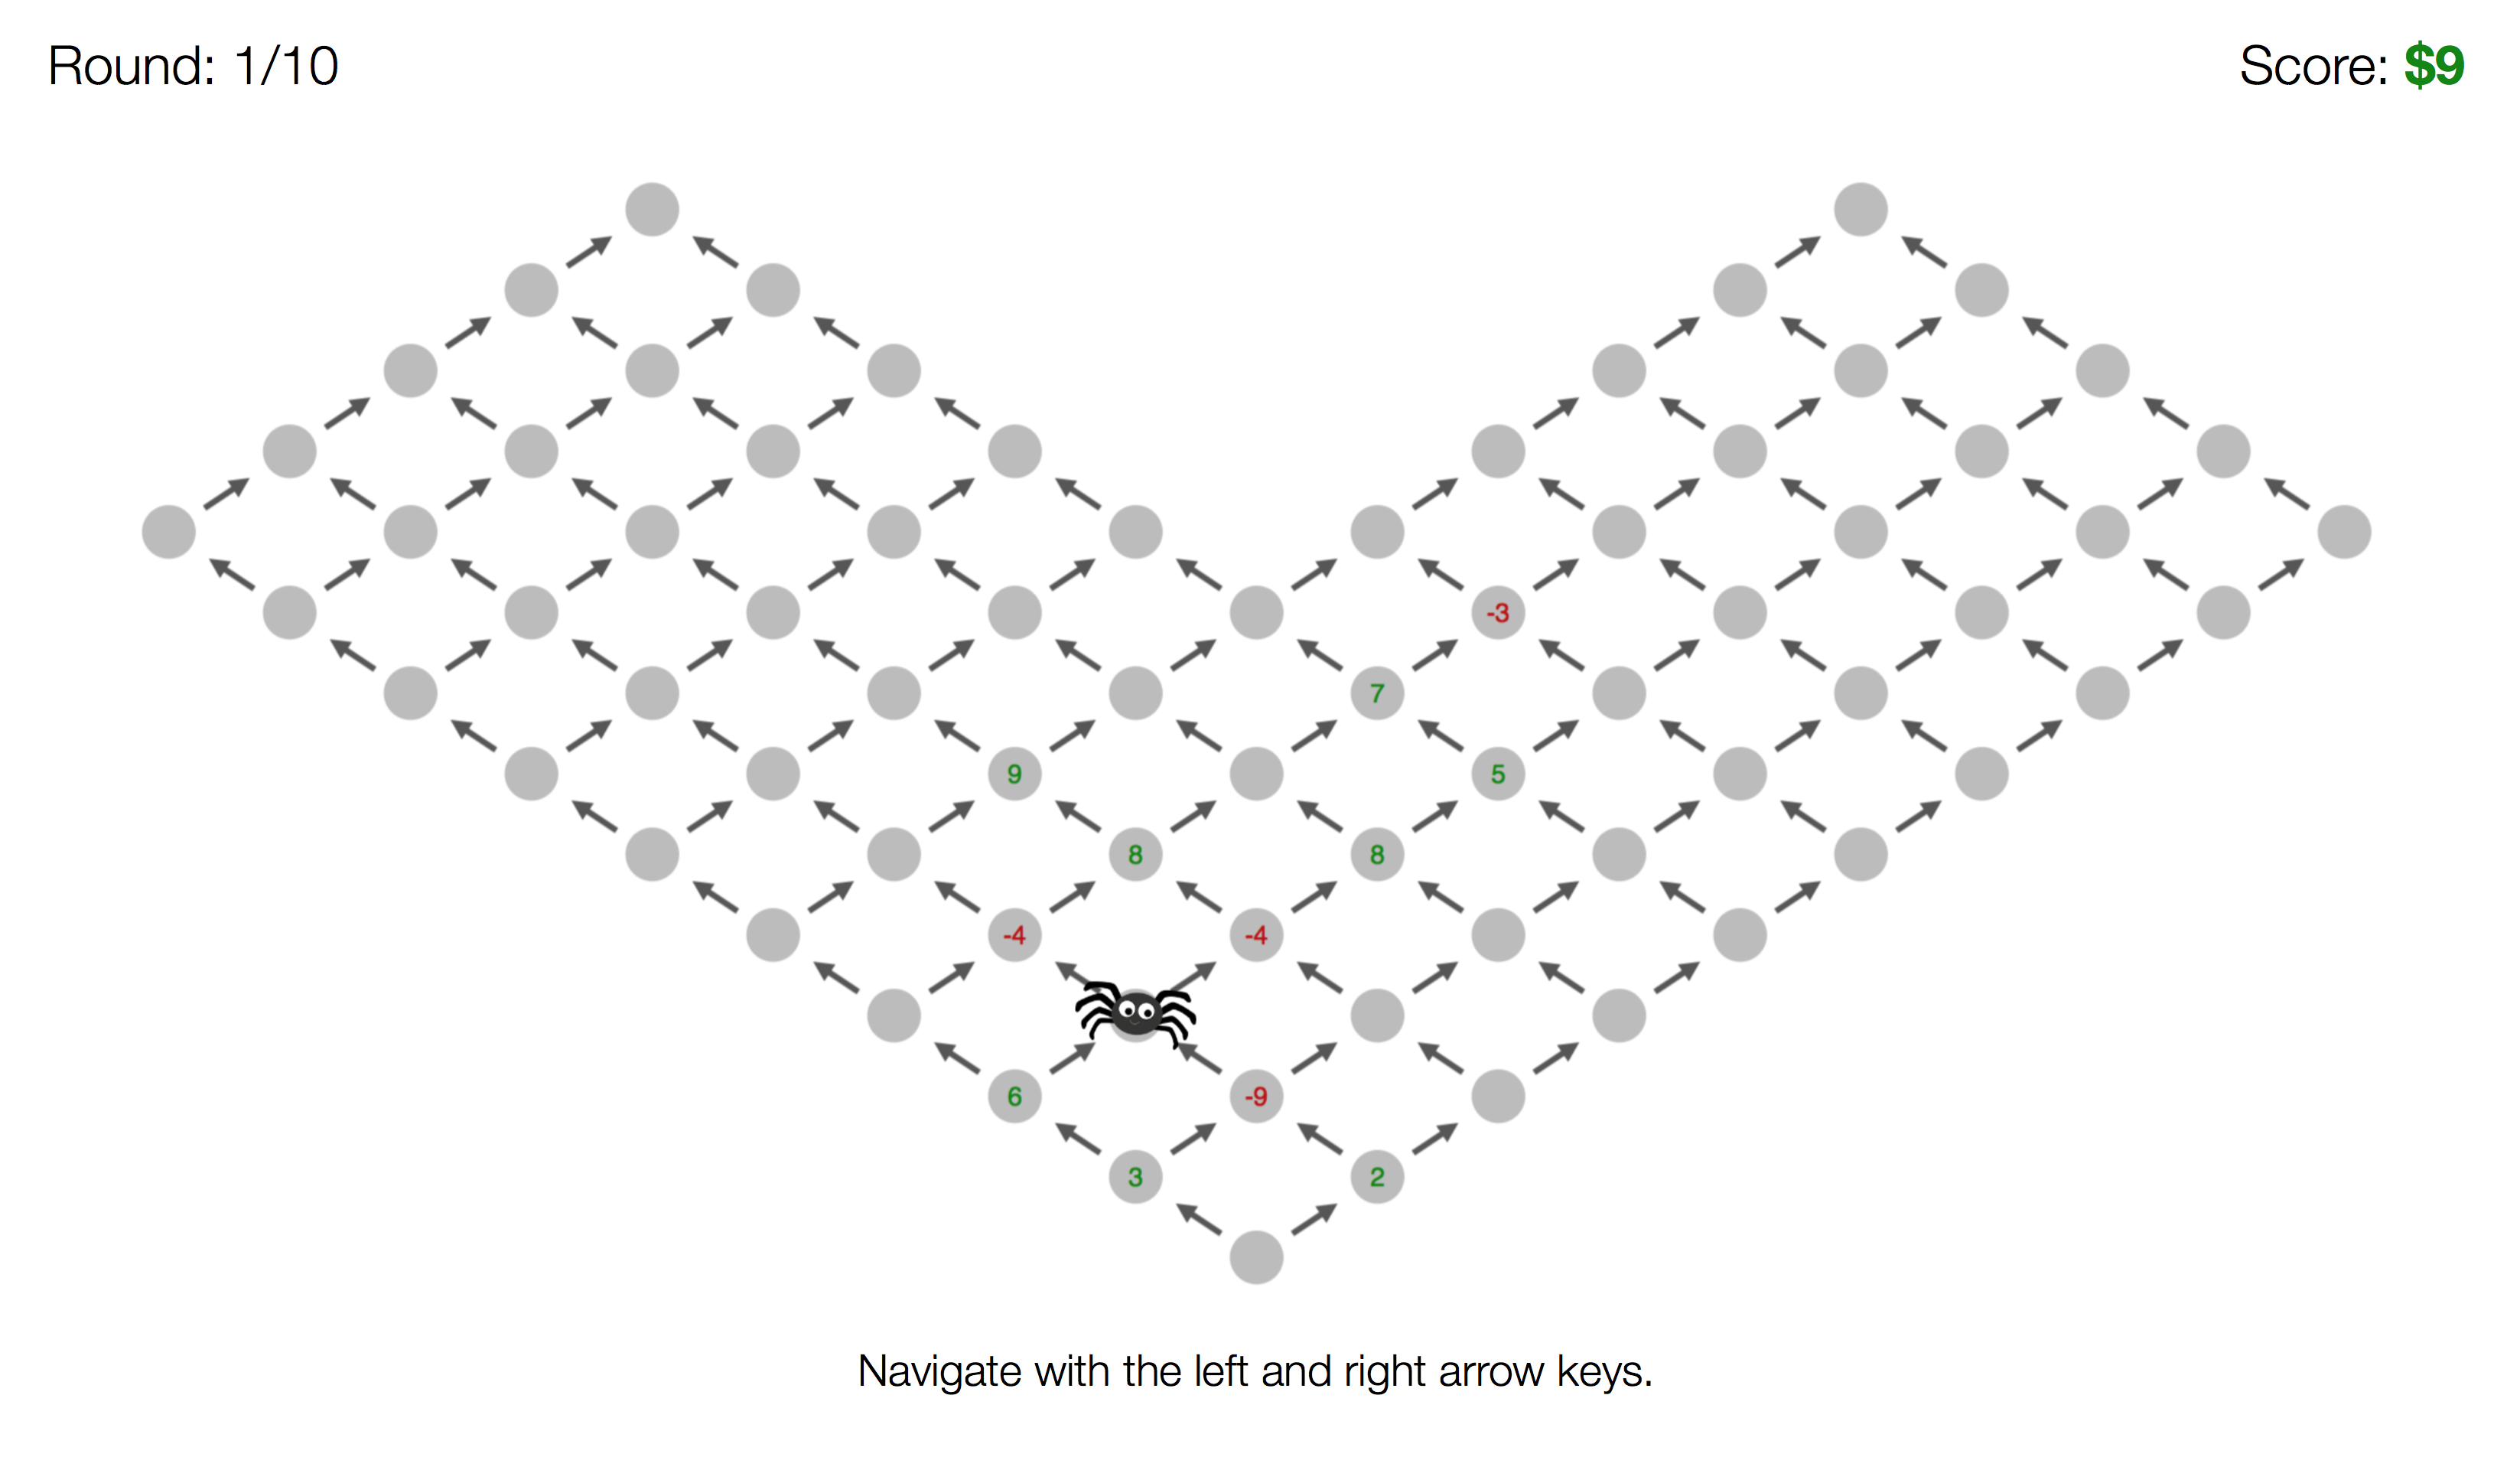
\includegraphics[height=10cm]{figs/heart.png}
  %     \captionof{figure}{Large environments can be programatically generated.}
  %     \label{fig:heart}
  %   \end{minipage}%
  %   \begin{minipage}{.3\textwidth}
  %     \centering
  %     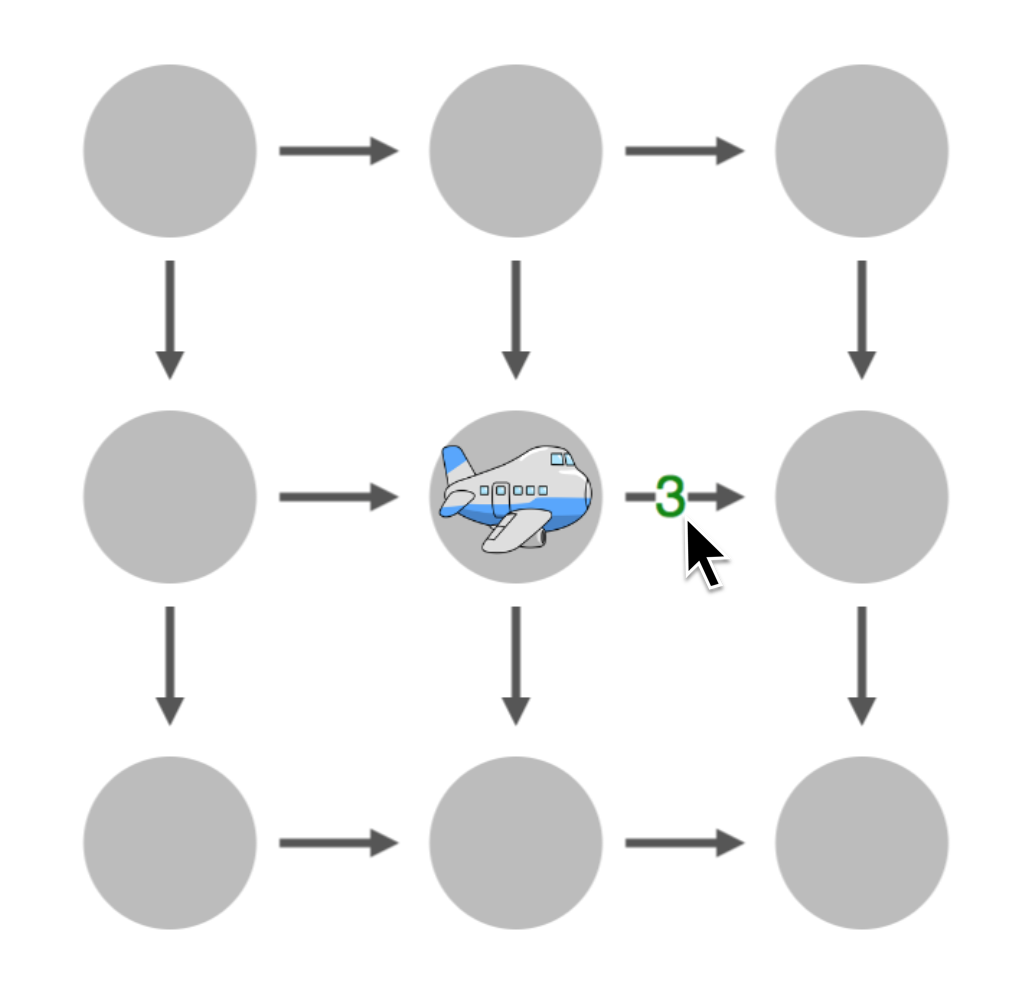
\includegraphics[height=10cm]{figs/grid2.png}
  %     \captionof{figure}{Rewards can be displayed always, after being clicked, or only on hover.}
  %     \label{fig:hover}
  %   \end{minipage}
  % \end{figure}



  % \begin{columns}[t,totalwidth=\twocolwid] % Split column 2 into 2.1 and 2.2
    
    % \begin{column}{\onecolwid} % Begin column 2.1
      
      

    % \end{column} % End column 2.1

  %   \begin{column}{\onecolwid} % Begin column 2.2


  %     % \begin{figure}
  %     %   % \label{fig:paradigm}
  %     %   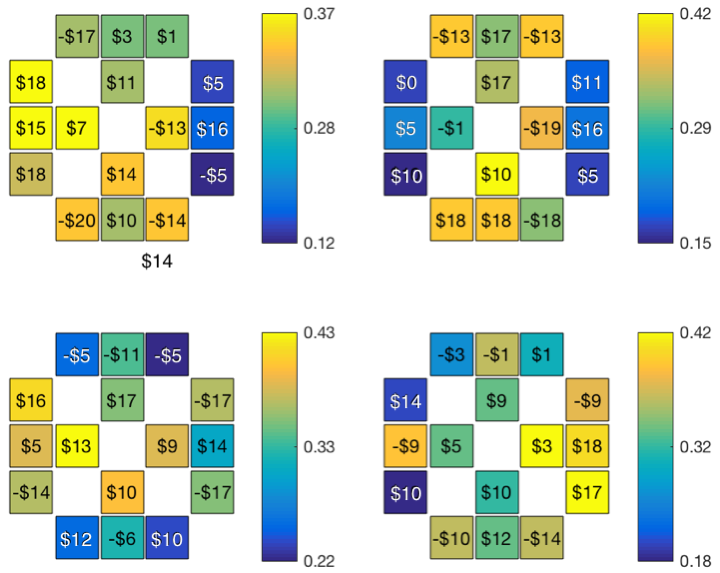
\includegraphics[width=0.9\linewidth]{figs/click_locations_noFB_before1stFlight_small.png}
  %     %   % \captionsetup{width=0.9\linewidth}
  %     %   % \caption[first]{Web of Cash experimental interface.}
  %     % \end{figure}
    
  %   \end{column} % End column 2.2

  % \end{columns}

\end{column} % End column 2
%------------------------------------------------------------------------------
\begin{column}{\sepwid}\end{column} % Empty spacer column
\begin{column}{\onecolwid} % Begin column 3

  \begin{block}{Experiment}\label{experiment}
    \begin{itemize}
      \item Proof-of-concept experiment run online ($N=31$)
      \item Layout encourages pruning (center image)
      \item Reward at each state revealed upon click
      \item \$0.10 penalty for each click
      \item Minimum of 45 seconds per trial
    \end{itemize}
  \end{block}

  \begin{block}{Results}\label{results}
    Clicking patterns provide \textbf{direct evidence of pruning}.
    \begin{itemize}
      \item Fewer clicks on states after large costs (Fig.~2)
      \item Effect varies smoothly with reward (Fig.~3)
    \end{itemize}
  \end{block}

  \begin{figure}
    \label{fig:pruning}
    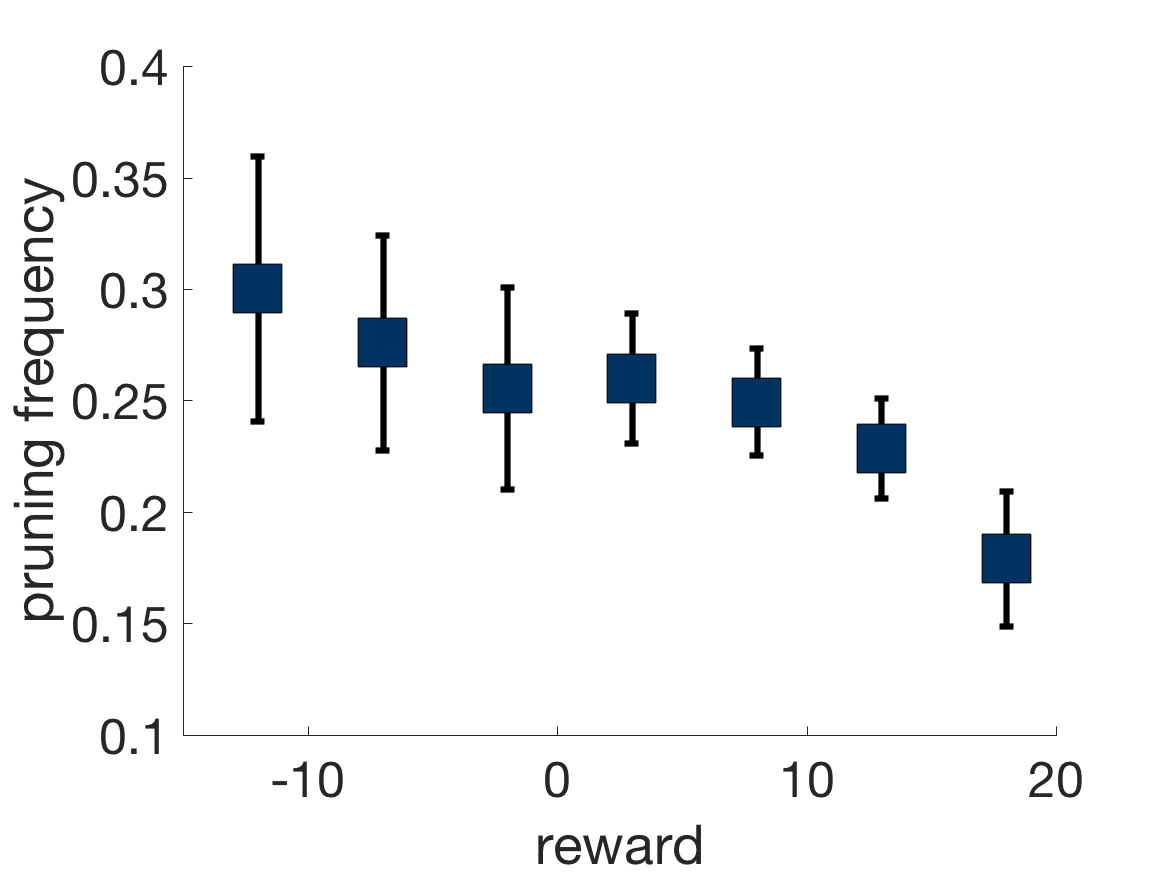
\includegraphics[width=0.9\linewidth]{figs/prunning_any_noFB.png}
    \captionsetup{width=0.9\linewidth}
    \caption[first]{Frequency of pruning $\pm 1 \text{SEM}$ given the reward at the stem of the branch. Pruning was defined as inspecting none of a branch's outer states (before the second move) after having inspected the reward at its stem (before the first move).}
  \end{figure}

  \begin{block}{References}\label{references}
    \bibliographystyle{unsrt}
    \tiny
    % \setlength{\bibleftmargin}{.05in}
    % \setlength{\bibindent}{-\bibleftmargin}
    \bibliography{references}
  \end{block}

  % \setbeamercolor{block title}{fg=red,bg=white} % Change the block title color

  % \begin{exampleblock}{Acknowledgements}
    \small{\rmfamily{\textbf{Funding}\; ONR MURI N00014-13-1-0341 and the Templeton World Charity Foundation.}}
  % \end{exampleblock}

  %\begin{flushright}
  %  \texttt{https://github.com/fredcallaway/Mouselab-MDP}
  %\end{flushright}

\end{column} % End column 3

\end{columns} % End of all the columns in the poster

\end{frame}

\end{document}
